\documentclass[12pt]{article}

\usepackage{graphicx}
\usepackage{caption}
\usepackage{subcaption}
\usepackage[spanish]{babel}
\usepackage[utf8]{inputenx}
\usepackage{anysize} 
\usepackage{amsmath}
\usepackage{listings}
\usepackage{wrapfig} % paquete gráfico... quizás es necesario actualizar paquetes en kile
\usepackage{hyperref}

\usepackage{fancyhdr}
\pagestyle{fancy}

\hypersetup{
    colorlinks,%
    citecolor=black,%
    filecolor=black,%
    linkcolor=black,%
    urlcolor=black
}
\marginsize{2cm}{2cm}{1cm}{1cm} %izq der arriva abajo

\title{Informe preliminar}
\author{Facundo Nahuel Uriel Silva}

\lhead{ \chaptername }

 
\begin{document}

  %Caratula
  \newpage
  \thispagestyle{empty}
  
  \begin{center}
    
\includegraphics[width=250px]{../../logo_fiuba_alta.jpg} 

  \vspace{100px}

  {\bf \huge{Trabajo Profesional de Ingeniería Electrónica} }
  
  \vspace{30px}

  \Large{Sistema de control para proceso de sinterizado de nano estructuras }
  
  \vspace{30px}
  
  \Large{\textit{Situacion inicial}} % ver que poner aca.....

  \end{center}

  \vspace{100px}

   \begin{bf}
    \begin{Large}
      \begin{tabbing}
	\= ----- \= ----- \= --------------------- \= \kill
	\> Integrantes:\\
	\\
	  \>\> Estanislao López Morgan \\
	  \>\>\>  Padrón:	\> 84546 \\
	  \>\>\>  Mail:	\>\url{estanux@gmail.com} \\
	\\
	  \>\> Facundo Nahuel Uriel Silva\\
	  \>\>\>  Padrón:	\> 86881 \\
	  \>\>\>  Mail:	\> \url{fanaur@gmail.com}\\
      \end{tabbing}
    \end{Large}
  \end{bf}



  %Indice de contenidos
  \newpage
  
  
  \thispagestyle{empty} \tableofcontents \thispagestyle{empty} %asi se sace el numero de pagina

  %Comienzo
  \newpage
  \setcounter{page}{1}
  
  \section{Introducción}
 Los materiales nanocompuestos formados en su totalidad por particulas cerámicas y metálicas en el rango de los centenares
 y decenas de nanómetros, son una clase de materiales que presentan propiedades físicas muy distíntas a las de esos mismos
 con tamaños de cristal micrométricos (materiales convencionales). Tales propiedades, al ampliar su rango de funcionalidad
 resultan muy interesantes desde el punto de vista tecnológico ya que permiten combinar propiedades excepcionales con funcionalidad
 imprescindibles en aplicaciones específicas, como la transparencia, la biocompatibilidad, la dureza o conductividad eléctrica, entre otras.

 Sin embargo, la aplicacion industrial de los materiales nanocompuestos radica en la capacidad de consolidación de estos materiales
 formando cuerpos densos y compuestos, pero preservando el tamañan nanométrico de sus componentes. Las técnicas de consolidación convencionales
 presentan importantes limitaciones y no son capaces de preservar esta nanoestructura. 
 La solución de estos problemas y el desarrollo de nuevas tecnologías ha posibilitado la producción de materiales nanoestructurales.

 En el laboratorio de sólidos amorfos de la facultad de ingeniería de la universidad de Buenos Aires funciona el 
 INTECIN y en el mismo el \href{''http://intecin.fi.uba.ar/grupos.php?grupo=12''}{grupo de materiales nanoestructurales}, este grupo prepara y
 estudia sistemas basados en nanopartículas magnéticas apuntando a las posibles aplicaciones tecnológicas
 en sensores, remediación ambiental y aplicaciones clínicas. Sus integrantes tienen experiencia en caracterización estructural por difracción, dispersión y absorción
 de rayos X, espectroscopia Mössbauer, propiedades magnéticas y de magnetotransporte y microscopía electrónica.\newline
  
 Para lograr esto se realiza el sintetizado de nano estructuras, obteniendo una cinta metálica con una estructura amorfa similar 
 a un vidrio. Mediante un proceso de
 pulverizado de esta cinta se obtiene un polvo cuyas partículas poseen una estructura nanométrica.
 Para poder obtener una estructura sólida a partir del polvo se utiliza el proceso de sinterizado. Este proceso
 logra unificar las particulas del polvo en una sola estructura sólida. Para este fin se necesita que una intensidad de corriente
 elevada, en el orden de los KA, atraviese la muestra de polvo nonometrico. Esta corriente puede ser provista por un banco de 
 capacitores (proceso rápido) o una fuente de RF (proceso lento).\newline

 La finalidad de nuestro proyecto es desarrollar una automatización y relevamiento del proceso de sinterizado a partir de la 
 descarga de un banco de capacitores, realizar recopilación de datos del proceso con la posibilidad de variar alguna variables
 involucradas en el sitenrizado para evaluar el desempeño del mismo y sus resultados.

 La finalidad de este informe es describir la situación existente en el laboratorio y plantear una posible solución tecnológicas 
 para el proceso de control.


  \newpage

  \section{Descripción situación existente del sistema}

  \begin{wrapfigure}{r}{0.50\textwidth}
      \vspace{-20pt}    
      \begin{center}
      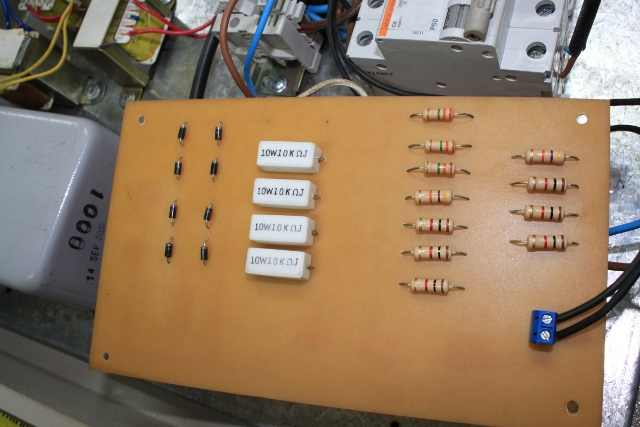
\includegraphics[width=0.49\textwidth]{../../Diagramas/FotosRelevamiento/RectificadoBacoRLR.JPG}
     \end{center}
    \caption{Tablero actual}
  \end{wrapfigure}
  
  En la actualidad, el antiguo proceso de sinterizado, que estuvo en funcionamiento a modo de prueba para realizar solo algunas 
  descargas de los capacitores, se encuentra parcialmente desmantelada. 
  Se cuenta con una caja metálica que hace la suerte de tablero, alberga la electrónica de control y un pequeño teclado con un
  display de cristal líquido. Contiene también un contactor y una placa con un puente de diodos, algunas resistencias pequeñas y un rele.

En el laboratorio se encuentran dos capacitores de potencia en derivación marca Leyden. Son de 200uF por 1000V y tienen un dieléctrico constituido en general por tres películas de polipropileno ‘hazy’, 
rugosas en ambas caras, de alta pureza. Esta construcción, en lugar de la que utiliza sólo dos capas de un film rugoso en una sola de sus caras, común en otros fabricantes, ``confiere a los capacitores
LEYDEN mayor seguridad de funcionamiento y mayor vida útil. La rugosidad en ambas caras del polipropileno es una condición indispensable para la completa impregnación
del film durante el proceso y, por ende, para la estabilidad del capacitor a largo plazo'', especifica el fabricante. \newline

Estos capacitores utilizan un impregnante no-clorado MDBT. Éste se caracteriza por su alto punto de inflamación, gran capacidad de absorción de gases derivados de descargas eléctricas internas,
 y compatibilidad ambiental (biodegradabilidad).

  \begin{figure}[h!]

    \begin{subfigure}[b]{0.5\textwidth}
      \centering
      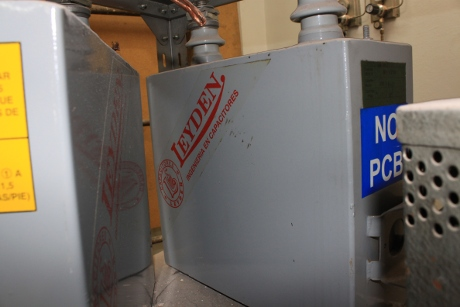
\includegraphics[height=150px,keepaspectratio=true]{../../Diagramas/FotosRelevamiento/CapacitoresDeLadoLR.JPG}
      \caption{Capacitores de lado}
    \end{subfigure}
    ~
    \begin{subfigure}[b]{0.5\textwidth}
      \centering
      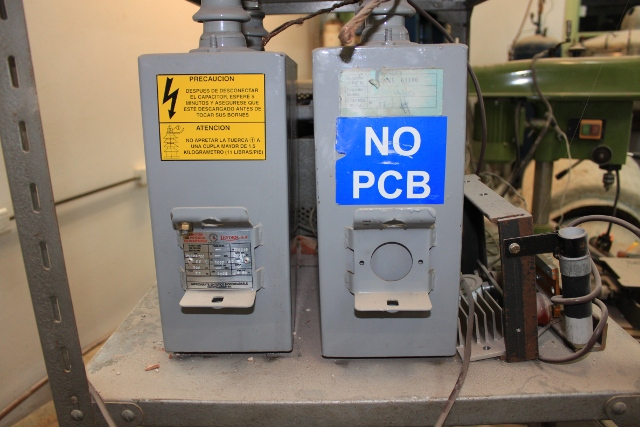
\includegraphics[height=150px,keepaspectratio=true]{../../Diagramas/FotosRelevamiento/CapacitoresLR.JPG}
      \caption{Capacitores de frente}
     \end{subfigure}
    ~
    \caption{Capacitores de 200uF y 1000V}

  \end{figure}

% 
%   \begin{wrapfigure}{l}{0.52\textwidth}
%       \vspace{-20pt}    
%      \begin{center}
%       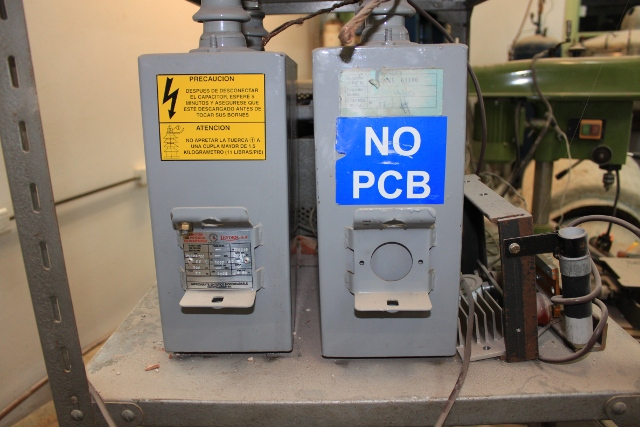
\includegraphics[width=0.50\textwidth]{../../Diagramas/FotosRelevamiento/CapacitoresLR.JPG}
%      \end{center}
%     \caption{Capacitores}
%   \end{wrapfigure}

%\vspace*{300px}
  

\newpage

\section{Descripción solución propuesta}

\subsection{Objetivos}
  
  Se propone desarrollar un sistema electrónico que integre el control y la adquisición de datos del proceso de sinterizado ECAS (Electric current activated/assisted
  sintering ). La corta duración del proceso de descarga de los capacitores (razón por la cual a esta modalidad se la denomina 'ultra rápida')
  exige que el sistema tenga una elevada velocidad de respuesta para tomar las muestras de las distintas magnitudes físicas que se necesitan medir en el proceso.
  El sistema utilizará la información provista por los sensores para hacer ajuste en los parámetros de control del proceso para lograr los mejores resultado 
  en experimentación.
  Se estimara la carga del banco de capacitores para de esta manera saber con precisión la magnitud que tendrá la corriente en el momento de la descarga,
  siendo este aspecto de fundamental importancia en este proceso.
  El proceso requiere la presencia de altas tensiones para su ejecución por lo que el sistema monitoreará todos los parámetros peligrosos (como son tensión de la fuente
  de alimentación y la tensión de los capacitores) y aplicara todas las medidas de seguridad necesarias para brindarle al operador la seguridad necesaria
  para su utilización. El sistema tendrá la capacidad de poder interrumpir el proceso en caso de no ser seguro para el operario o para la integridad de los elementos
  del sistema (para evitar daños). El sistema contara con indicadores lumínicos (luces de señalización) y sonoros (sirenas) para informara los distintos
  estados del sistema.
  Los datos obtenidos de la experimentación podrán ser accedidos desde distintos medios para facilitar el posterior análisis de la información recolectada.
  Se tendrá un acceso remoto al sistema mediante la conexión a una red local (LAN) y un acceso local mediante la interfase provista por el teclado y la pantalla.
  En la figura \ref{fig:ECAS control} se muestra de forma esquemática los componentes que integraran al sistema. Se tendrá una unidad de control acompañada de
  un conjuntos de sensores y actuadores.

  \begin{figure}[h!]
      \centering
      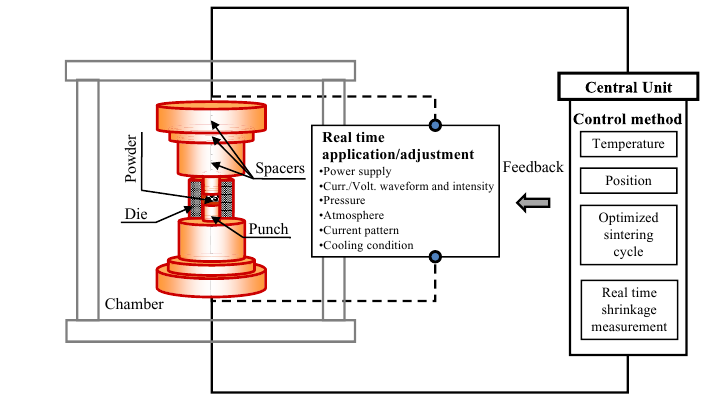
\includegraphics[height=250px,keepaspectratio=true]{../../Diagramas/ECAS_control.png}
       \caption{Descripción general del proceso ECAS}
      \label{fig:ECAS control}
  \end{figure}

  \newpage

  \subsection{Diagrama en bloques}

    Se muestra en la figura \ref{fig:DiagramaBloqueGeneral} los bloques funcionales principales que compondrán el sistema planteado.
  
    \begin{figure}[h!]
      \centering
      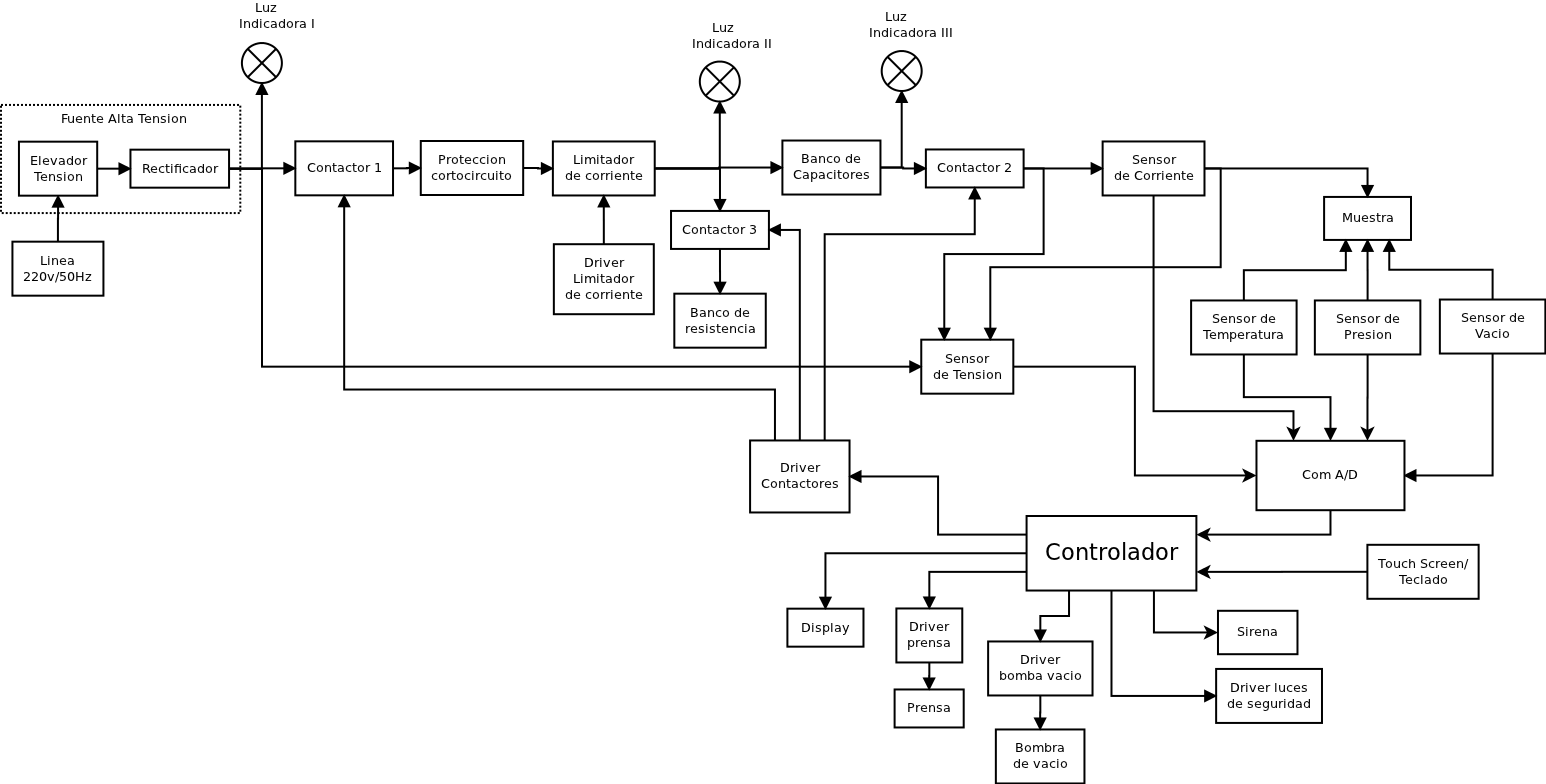
\includegraphics[height=315px,angle=90,keepaspectratio=true]{../../Diagramas/diagramaBloquesMacro.png}
      \caption{Diagrama en bloque general del sistema}
      \label{fig:DiagramaBloqueGeneral}
    \end{figure}

  \newpage

  \subsection{Descripción en bloques funcionales del sistema}    
  
  Se han agrupado funcionalidades de forma de poder modelizar el sistema total como la interconexión de bloque que cumplen funciones muy especificas
  dentro del funcionamiento general. Se detalla a continuación la función de cada bloque:

  \begin{itemize}
    \item Fuente Alimentación: Este bloque esta encargado de tomar la energía de la red de alimentación en forma de tensión alterna y transformarla en 
				tensión continua de alta tensión para que sea adecuada para cargar los capacitores de 1000v. 
    \begin{itemize}
      \item Elevador: Este sub bloque de la fuente de alimentación tiene la tarea de elevar la tensión proveniente de la linea de alimentación de 220v 
		      hasta los 1000v.
      \item Rectificador: Este bloque transforma la tensión alterna de 1000v a una tensión continua de 1000v mediante la rectificación y el filtrado de la tensión
			  de entrada.
    \end{itemize}

    \item Luz indicadora: Este bloque provee al operador del sistema la posibilidad de visualizar la presencia de alta tensión para tomar así las precauciones necesarias.
    
    \item Contactor 1: Este bloque separa la fuente de alimentación de alta tensión del resto de sistema. El contactor se activará para permitir que la corriente
		      proveniente de la fuente de alta tensión cargue a los capacitores a la tensión indicada.
    
    \item Protección corto circuito: Este bloque es un mecanismo de protección que tiene la función monitorear la corrientes en caso de que se produzca un aumento
				      desmedido de la misma y en caso de detectarse esta situación procederá a la desconectara la alimentación del sistema
				      para evitar daños y se notificara la situación.
    
    \item Limitador corriente: Este bloque brinda al sistema la capacidad de poder controlar la corriente con la que cargan de los capacitores.
    
    \item Driver limitador corriente: Este bloque es el encargado de comandar el limitador de corriente.

    \item Contactor 3: Este bloque brinda la posibilidad de conectar eléctricamente un banco de resistencias para ser utilizado en caso de tener la necesidad de
			realizar la descarga de los capacitores si estos quedan con carga.

    \item Banco de resistencias: Este bloque esta compuestos por un conjunto de resistencias auxiliares que serán utilizados en caso de que los capacitores quedaran
			   con carga y se necesita que sean descargados por cuestiones de seguridad.

    \item Banco de capacitores: Este bloque esta compuesto por un conjunto de capacitores de alta tensión que son utilizados para almacenar cargar eléctricas.
				Una vez alcanzado el nivel de carga necesario para realizar la descargar los capacitores quedaran cargado hasta que se inicia el 
				proceso de descarga. En ese momento todas las cargar almacenadas en el bando de capacitores sera conducida hacia la muestra 
				de nano polvos para realizar el sinterizado de la muestra.
				
    \item Drivers contactores: Este bloque tiene como función actuar como interfase entre la lógica de control y los contactores.

    \item Contactor 2: Este bloque tiene como función conectar eléctricamente los capacitores con la muestra una vez que se han cargado los capacitores al nivel de
			de carga requerido.

    \item Sensor tensión: Este bloque es un transductor utilizado para medir la tensión de la fuente de alimentación y la tensión que poseen los capacitores para 
			    así poder inferir la carga que poseen. 
    
    \item Sensor de corriente: Este bloque es utilizado para la medición de la corriente que circula al momento de la cargar de los capacitores y para relevar la
			      corriente circulante a la hora de la realización de la descarga de los capacitores.

    \item Muestra: Este bloque indica donde se encontrara la muestra compactad de nano polvos la cual sera expuesta a la descarga de los capacitores.

    \item Sensor temperatura: Este bloque tiene como fin relevar la evolución de la temperatura de la muestra durante la descarga de los capacitores sobre la muestra.

    \item Sensor presión: Este bloque relevara la presión mecánica ejercida sobre la muestra de nano polvos.
    
    \item Sensor de vacío: Este bloque relevara el nivel de vacío que se tiene en la zona donde se encuentra la muestra. Este bloque se utilizara en el caso de 
			    que se utilice una cámara de vacío para realizar el proceso.

    \item Conversor A/D: Este bloque tiene la función de digitalizar los niveles de tensión y/ó corriente provenientes de los sensores del sistema para poder
			  ser interpretados y utilizados por la lógica de control del sistema.

    \item Touchscreen/ Teclado: Este bloque brinda un medio para el accionamiento del sistema por parte del usuario.

    \item Sirena: Este bloque tiene como fin la indicación sonara de un estado, ya sea de aviso o para indicar un problema.

    \item Driver luces de seguridad: Este bloque tiene como función actuar como interfase entre la lógica de control y las luces de señalización.

    \item Driver bomba de vacío: En caso de necesitarse una nivel de vacío para el proceso este bloque funcionara como interfase entre la lógica de control
				  y la bomba de vacío.

    \item Bomba de vacío: Este dispositivo tiene como fin producir el nivel de vacío necesario par el proceso en la cámara de vacío donde se encuentra la muestra de
			  nano polvos.

    \item Driver prensa:  Este bloque tiene como función actuar como interfase entre la lógica de control y la prensa mecánica que comprime la muestra de nano polvos.

    \item Prensa: Este bloque tiene la función de ejercer una fuerza mecánica en los extremos de la muestra de nano polvos para poder asegurar un buen contacto
		  eléctrico durante el proceso de descarga de los capacitores sobre la muestra.

    \item Display: Este bloque brinda un medio para la señalización al usuario de indicadores del proceso.

    \item Controlador: En bloque esta la lógica de control y comunicación del sistema. La lógica se ocupa tanto al control y accionamiento de los periféricos
		      del sistema como del almacenamiento y procesamiento de los datos obtenidos. Este bloque también es el responsable de brindarle al sistema
		      la comunicación con el usuario ya sea mediante red , dispositivo de almacenamiento extraíble o mediante el teclado/touchscreen y el display.

  \end{itemize}


%   \subsection{Conectividad}    
% 
%     \begin{figure}[h!]
%       \centering
%       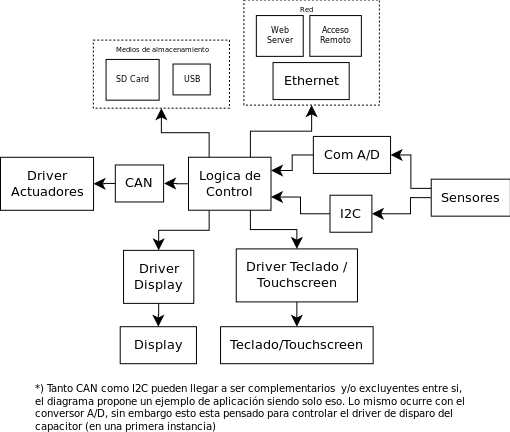
\includegraphics[width=400px,keepaspectratio=true]{../../Diagramas/microEsquema.png}
%       diagramaBloquesMacro.png: 1546x783 pixel, 72dpi, 54.54x27.62 cm, bb=0 0 1546 783
%       \caption{Diagrama en bloque de la logica}
%       \label{fig:DiagramaBloqueLogica}
%     \end{figure}


  %Bibliografia
  \newpage

  \begin{thebibliography}{1}
    \bibitem{ ECAS_tecnologys_page } \url{ http://iopscience.iop.org/1468-6996/10/5/053001 }
    \bibitem{ ECAS_tecnologys_pdf } \url{ http://iopscience.iop.org/1468-6996/10/5/053001/pdf/1468-6996_10_5_053001.pdf }
    \bibitem{ ECAS_wiki } \url{ http://en.wikipedia.org/wiki/Capacitor_discharge_sintering }    
    \bibitem{ Capacitores Leyden } \url{ http://www.leyden.com.ar/esp/index.html }

  \end{thebibliography}
    

\end{document}